
\documentclass[letterpaper,twocolumn,10pt]{article}
\usepackage{usenix-2020-09}

% to be able to draw some self-contained figs
\usepackage{tikz}
\usepackage{amsmath}

% inlined bib file
\usepackage{filecontents}

% to include png figures
\usepackage{graphicx}

% Include the listings package and define code style
\usepackage{listings}
\lstdefinestyle{mystyle}{
    language=Python,
    basicstyle=\ttfamily,
    keywordstyle=\color{blue},
    commentstyle=\color{green},
    stringstyle=\color{red},
    breaklines=true,
    showstringspaces=false,
    numbers=left,
    numberstyle=\tiny,
    frame=single
}

%-------------------------------------------------------------------------------
\begin{document}
%-------------------------------------------------------------------------------

%don't want date printed
\date{}

% make title bold and 14 pt font (Latex default is non-bold, 16 pt)
\title{\Large \bf CYBR410 Group Project: Big Deployment}

%for single author (just remove % characters)
\author{
  {\rm Paul Aguilar}\\
  Front-End
  \and
  {\rm Nehemiah Fiedls}\\
  Logging
  \and
  {\rm Eric Leachman}\\
  Orchestration
  \and
  {\rm Thomas Longwell}\\
  Defense
  \and
  {\rm Robert Rutherford}\\
  Defense
  \and
  {\rm Spencer West}\\
  Services
  \and
  {\rm Nicholas Burlakov}\\
  Services
}

\maketitle

%-------------------------------------------------------------------------------
\begin{abstract}
%-------------------------------------------------------------------------------
The goal of this project is to work as a group with each member implementing a different aspect making up a larger deployment. The end goal is a secure and easily accessible web server with an aesthetic front end, useful services such as an IP to physical location and an IP to weather converter, a robust defense to deter attackers,  and a method to log all traffic on the server. 
\end{abstract}


%-------------------------------------------------------------------------------
\section{Introduction}
%-------------------------------------------------------------------------------
This project is designed to have groupmates work together to design and implement a full deployment. Each team mate was assigned a specific piece of the deployment as their responsibility and each section of this paper relates to a section of the deployment. Front-End is in charge of creating the user interface of the deployment as well as the web server that will host the services. The Services team then implemented an URL to physical location feature as well as a URL to current weather forecast converter. Behind the scenes the Defense team integrated an IP blocking honeypot to deter attacks, while Logging used a Sysdig script to keep a record of all traffic. This was handed to Orchestration, who spun up the servers on the designated IP assigned by the professor. 


%-------------------------------------------------------------------------------
\section{Related Work}
%-------------------------------------------------------------------------------
	In a basic connection between a client and a host, one computer would send a request that would get relayed by a server to the destination computer. In a proxy environment, the proxy sits in the middle between the client and the server, relaying the requests to the server on the client's behalf. One defense implementation used in this project is a reverse proxy. Unlike a forwarding proxy, which forwards network traffic on your behalf, a reverse proxy forwards traffic to a specific destination, usually you. They are positioned in front of web servers and forward browser requests to those servers. This is typically done for a few reasons, including load balancing, cyber defense, caching, and even SSL encryption\cite{CloudFlare_2024j}. A load balancer is used to distribute traffic among several servers, preventing direct traffic from overloading any given one, like a mail room. In terms of defense, it obfuscates a client's actual IP address, making it a more difficult target; and ideally, the reverse proxy is a third-party that has the infrastructure to defend against attacks. 

	For this project, rather than use a third-party company to act as a reverse proxy, a software tool called NGINX was employed. NGINX is a free, open-sourced web server released in 2004 that can be used as either an HTTP, reverse proxy, mail proxy, and generic TCP/UDP proxy server. It is popular and dependable enough to be used by major companies like Netflix and Dropbox. In fact, it is one of the top four most used services, and incredibly popular in the Docker community as the most commonly deployed technology in docker containers\cite{wikiNginx_2024m}. For this reason, it made it an easy choice when looking for a technology to act as the project's reverse proxy that could be easily incorporated into our Docker implementation. 

	Honeypots are widely used tools that can provide invaluable data when in a defensive position. In general, they’re decoys that lure attackers in to allow a defensive team to study the incoming attacks. In this project specifically, the network service daemon OpenCanary has been implemented\cite{OpenCanary_2024j}. Major benefits of this implementation are its extremely low resource requirements and the easy extensibility. It can be a good way to get IPs scanning networks, as the only case it should be discovered is if someone is scanning the entire network searching for vulnerabilities. Use of this stemmed from a want to diversify the implemented defensive techniques. By incorporating OpenCanary it has allowed greater surface from which logs can be collected which is extremely valuable for an evolving defense. Additionally, malicious IPs can be identified more regularly, presenting the opportunity to create IP blocking rules in the future. 


%-------------------------------------------------------------------------------
\section{Threat Model} \label{Threat Model}
%-------------------------------------------------------------------------------
\input{threatmodel}

%-------------------------------------------------------------------------------
\section{Orchestration}
%-------------------------------------------------------------------------------
The orchestration for this deployment concerns itself with two key areas. The first area, services, 
have been designed utilizing docker containers and docker compose for simple build up and tear down. 
Our docker compose solution utilizes two docker images, one running NGINX as a reverse proxy, 
and the other running a flask server locally which serves as an endpoint for the NGINX server. 

The second area, defense, utilizes OpenCanary and IPTables. While OpenCanary is also a docker container, the 
complexity in building it warrants its own separate orchestration. To accomplish this, we utilize 
some basic bash scripting to automate the necessary commands to run OpenCanary with the configuration and 
services required. We also include IPTables commands part of this bash script. These rules filter ports and 
drop traffic that attempts to enumerate OpenCanary and its ports. 

By automating most of the more complex tasks, our services and defenses can be deployed quickly 
and by a greater number of individuals, even those not intimately familiar with its inner workings. 
The use of docker containers and docker compose also allow our deployment to be mobile, only requiring 
prospective users to install a small number of programs (i.e., docker, docker compose, git). 




%-------------------------------------------------------------------------------
\section{Front end}

	The front end is designed around a few simple HTML template pages, stylized with a CSS style guide. There are three main templates and a variation on two – the first template is the index, a home page that is repeatedly linked on some blank links in the navigation bar. There are also two pages dedicated to the address and weather API’s. These pages have two versions, a search and an output template. The search template uses a simple form for the user to input a URL. The output template displays the results from the API call. These files are hosted via a flask server. \cite{grinberg2018flask}

	The flask server uses the render\_template and request objects to function seamlessly with the HTML and CSS. Following traditional directory organizations, a templates and static directory are used to hold those files for flask to access.
	\begin{verbatim}
	/app
    		- fServer.py
    	/templates
        - index.html
    	/static
		logo png’s
		/fonts
      	/styles
            	- style.css
	\end{verbatim}
Flask’s render\_template is used to display the correct HTML template in any given scenario, either from the hostWeather method or directly in the HTML links. The request object is used to handle the form submissions so that the user provided URL’s can be used by the API methods to generate the correct output. Both hostAddress and hostWeather use a similar method to pass the URL correctly depending on whether a POST request was made from a form submission, via requests request.form method or directly from the URL query string. From there the API methods are used to gather the data, which is the outputted using the render\_template method and displayed with in the output template.

% Include Python code snippet
\begin{lstlisting}[style=mystyle, caption=hostWeather method handles GET/POST requests, label=lst:python]

@app.route("/weather", methods=['GET', 'POST'])
def hostWeather():
    if request.method == 'POST':
        # Logic to handle form submission via POST request
        incomingHost = request.form['url']
    else:
        # Logic to handle GET request
        incomingHost = request.args.get('url', '')

    ipAddress = getIP(incomingHost)

    if checkCache(cacheW, incomingHost):
        weather = cacheW[incomingHost]
    else:
    	weather=getWeather(incomingHost)
    	addCache(cacheW, incomingHost, weather)

\end{lstlisting}

	While the host methods route to the correct output page, the remaining routes direct a user to the index or the search pages. The following sequence diagram shows the basic user interaction with the site:
\begin{figure}[htbp]
    \centering
    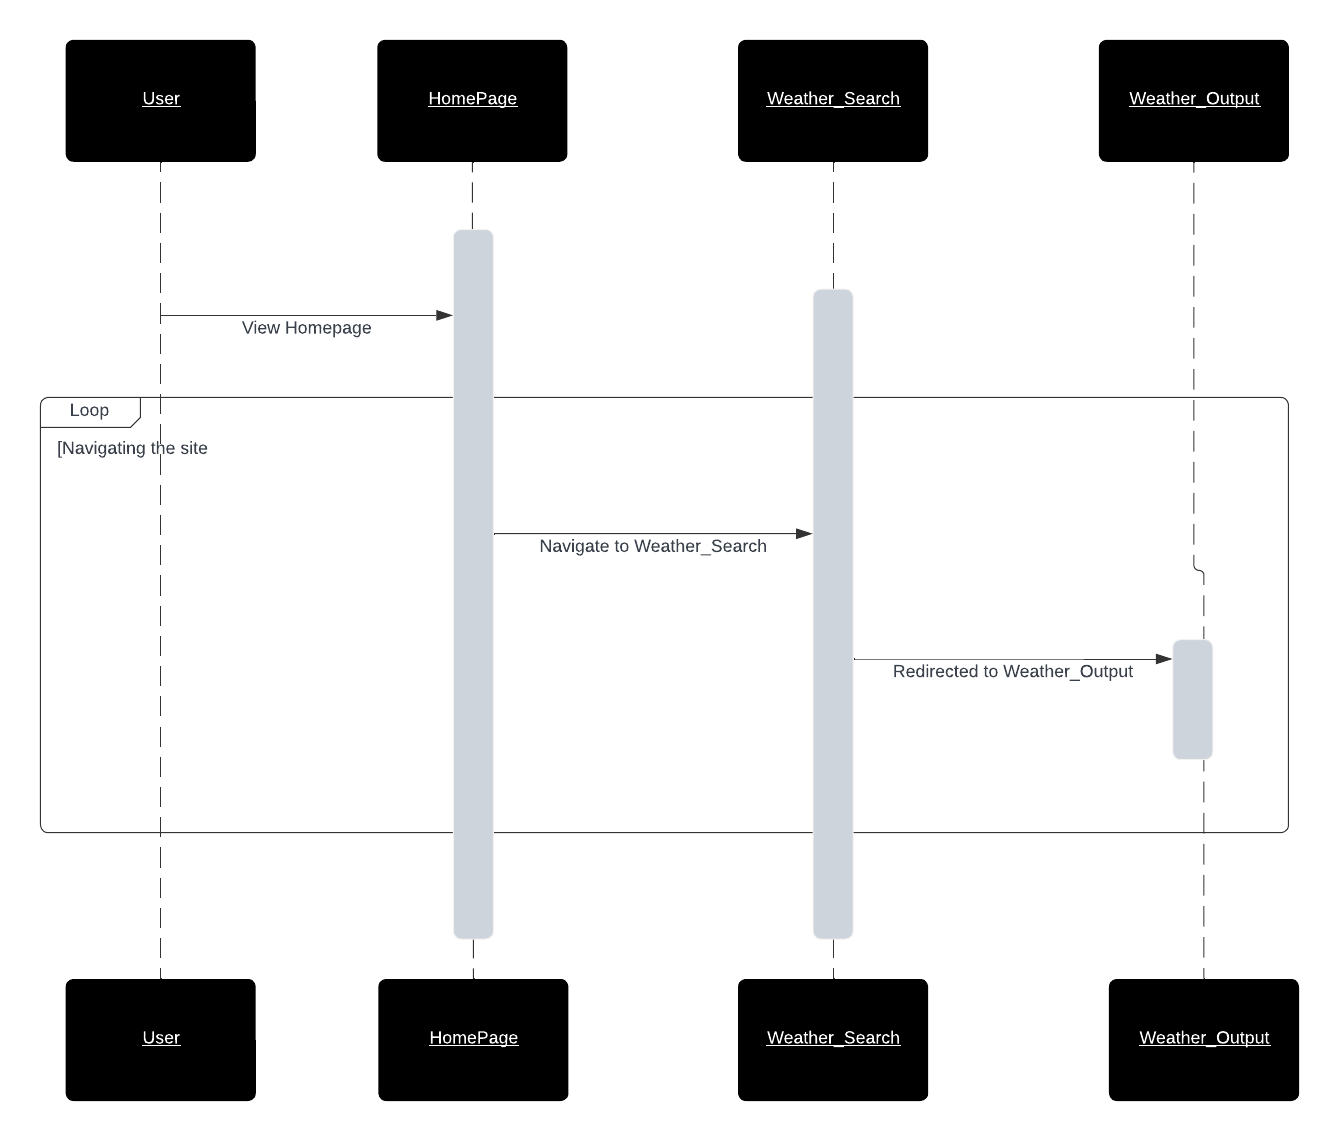
\includegraphics[width=0.5\textwidth]{sequenceD.png}
    \caption{Environment Diagram}
    \label{fig:example}
\end{figure}

%-------------------------------------------------------------------------------
\subsection{Evaluation Methodology \& Results}
%-------------------------------------------------------------------------------
\input{evalFrontend}
	

%-------------------------------------------------------------------------------
\section{Services}

	This web application incorporates two API's in a flask server. One service takes a URL and outputs the address of the registered owner based on the whois \cite{rfc3912} registry. The other uses that address and another weather API \cite{weather2009national,} to output the weather of that given location. It also uses a list to cache the data of visited sites, to improve performance. To do all this, the API is broken up in to multiple methods, which ultimately called by the hostWeather and hostAddress methods when a form submission is made on the webpage.
	
	The first method that is used is \verb+getIP()+, which first strips the incoming URL of any whitespace and then uses the socket library's \verb+gethostbyname()+ method to save the IP. This method is then used by both \verb+getWeather()+ and \verb+getAddress()+ in order to find the related information. \verb+getAddress()+ uses the subprocess' \verb+getstatusoutput()+ method to run the \verb+whois+ commandline tool to search for the registrar information based on the provided IP. It then splits the incoming tuple by a newline and parses out the different address fields, combines them and returns a whole address. 
	
	The getWeather method then passes that address in to a geocoding API to find the latitude and longitude of the address, which is required by the weather API that is used. The geocoding call returns a json file, that needs to be parsed and split between x and y coordinates correctly. The request's get method is then used to make an API call to weather.gov \cite{weather2009national} via the command line again. This outputs another json file that is then parsed to find the correct URL that contains the weather information. The get method is used once again on that forecast URL, which outputs the final json file, this is correctly parsed and returned as the weather for the given IP.

	The remaining methods handle the caching, either directly adding to it based on the correct list or traversing it to search for the given key which returns true or false. The host methods use this to first check the cache and then output the value based on the given key or add the key/value pair to the given cache if it isn't found. To summarize, this script creates a Flask web server that provides endpoints for IP address lookup and weather information retrieval, caching the results to improve performance. It also demonstrates how to integrate external APIs and system commands into a Flask application.


%-------------------------------------------------------------------------------
\section{Logging}

This is the logging section (miah)

%-------------------------------------------------------------------------------
\section{Defense}

In this section we will discuss the implementation of defense for our group project in detail. Our group's approach to defense includes a two part system, consisting of a honeypot and iptable rules to control traffic. The goal of the honeypot is to provide an avenue for investigation that distracts from the actual critical infrastructure. Once this unauthorized traffic occurs, the rules that we created drops the connection. This slows down or may entirely stop unauthorized users who have the intent to scan the server and try to connect or exploit it. With fake services on the honey pot, their attention will be diverted to multiple red herrings. This defensive approach assumes authorized users will know what is in scope and not try to connect to or scan the honeypot.

The honeypot we chose for this project is opencanary. Opencanary was selected because of our  familiarity with it, as well as its simplicity and interoperability with the rest of the group's implementation. It slots in easily because it’s built with docker, and allows our group to seamlessly integrate it with our other dockerfiles. This allows for quick configuration, and once the configuration file is set, building and running the dockerfile is easy. The ease of deployment works perfectly for the attacks that we anticipate later in the project, and will allow transferring of the honeypot to a new server to be easily handled with a single script. 

Traffic rules set by iptables include a very basic approach to discouraging traffic on the machine. Opencanary has enabled a large volume of ports that seem promising to exploit. After an initial scan, the attacker would recognize these and begin to press on these attack surfaces. Unbeknownst to them, all traffic going to these ports will be dropped with no reason or message given to the attacker. Using DROP instead of REJECT provides the client no insight into why their connection is unsuccessful. On their side, it just appears that their request is hanging forever. This simple yet effective measure is a major piece of our defensive strategy. Opencanary’s large volume of unnecessary ports in tandem with these rules will cause major disruptions to any penetration attempts, guaranteeing a strong level of security for the system. 



%-------------------------------------------------------------------------------

%-------------------------------------------------------------------------------
\section{Evaluation}

To evaluate our services, we opted to focus on the usability of our platform and its services as well as its security.
Focusing on the usability aspect allows us to approach from a user-perspective. We are concerned with bugs,
ensuring products are running appropriately, and ensuring that the interface is not broken. While focusing
on security related aspects, we focus our efforts based on our threat model.

For usability and service evaluation, we approached our deployment from the front end. Input fields were
tested for usability and for improper input. All links were tested on all page redundantly to ensure consistent
usability. All services were tested with proper and improper input.

Security evaluation of our deployment was done by engaging with our threat model to determine what knowledge
and tools are available to our adversaries. Knowing these key points allow us to accurately emulate the
types of enumeration and attacks we might see on our systems, allowing us to patch security vulnerabilities.
We evaluated our systems from all points that an aggressor will have access to, including the front end and
any services revealed via enumeration.

We first enumerate the IP address the deployment is located at, as we know that the aggressors in our threat
model will likely initially approach the system via this method. After establishing that the machine is online
utilizing Internet Control Message Protocol \hyperlink{https://datatracker.ietf.org/doc/html/rfc792}{(ICMP)} pings,
we then enumerate services and ports using the network mapper \hyperlink{https://nmap.org/}{Nmap}. After recording
the results of Nmap, we then perform enumeration with another CLI program, \hyperlink{https://github.com/OJ/gobuster}{Gobuster}.
Gobuster will map out the directory structure of machine giving us insight into what attack vectors might be exposed
to any aggressors.

With enumeration completed we know open ports, services offered, service versions, and directory structure, allowing
us to probe more deeply into individual components for vulnerabilities. This included probing SSH for vulnerabilities
and attempting access to our SQL server.

Investigation into some of the ports causes lots of confusion. Any non conventional port access is met with hanging requests when using curl or wget to access the web page. Further attempts to access these in a browser are met with the same results. While Nmap does show that those ports are open, it’s unable to detect exactly if there’s something blocking traffic. 

Our group also evaluated our logging by purging old logs that aren't necessary, as we wanted to clear the logs to clarify what traffic is produced by the expected attack referenced in the threat modeling section \ref{Threat Model}. Once the logs were purged our group ran a Nmap scan to generate traffic that would be captured using our logging. The Nmap scan used was \texttt{sudo nmap -T4 -A -sC 10.102.67.18}.




%-------------------------------------------------------------------------------
%-------------------------------------------------------------------------------
\section{Results}

After combining all components into a final working network with a web app with multiple services, the next stage was to analyze each of the services. 
Analyzing the services (otherwise known as enumeration) is the first step that a malicious actor might take. Using surveillance tools 
such as nmap, gobuster, or a ping sweep to map the hops of the system to checking what ports are available. One thing to note is that the tools listed 
are not exclusively used by malicious actors but are used by admins to provide better Cybersecurity solutions which is what the researchers of this 
study are applying.

We utilize nmap, a command line tool to determine what ports and services are currently on offer on a system,   
with the \verb|-sC| and \verb|-sV| flags which, respectively, will gather detailed information and the version that a service is operating on the network. In the 
study, the services are revealed as well as what ports those services operate on. For example it can be observed that there is an OpenSSH service 
operating on port 22 using tcp. A Defensive measure to protect this service would be to look at the \hyperlink{https://cve.mitre.org/}{CVE} (Common 
Vulnerabilities and Exposures) for OpenSSH. Looking at the CVE for OpenSSH, if the service is the most updated version, then admins might try to defend the encrypted 
key protocol to prevent messages from being deleted.

The ports that were revealed through an nmap scan also show that there is little security in protecting routing. This was observed as typing the port 
number at the end of the url such as “:9000” would reveal a webpage that had a scramble of letters and characters. This vulnerability could be remedied 
through proper routing controls so that url redirection attacks are minimized. In addition to eliminating security threats, testing was implemented on 
SSH for weak passwords. Passwords that were identified as weak were changed.

The iptable rules proved relatively effective in minimizing what could be discovered on the server. While they are found to be open with an nmap scan, they do drop all traffic that attempts to connect to them. By adding this element to the server we provide more opportunity for distraction and make it significantly more difficult to find something of value to an attacker. 

After testing our logging we found that former logs needed to be purged to make traffic from the expected attack clearer so we did so. After running the Nmap scan to generate traffic to test as referenced in the Evaluation section \ref{Evaluation} we found that our logs had produced multiple logs which when analyzed had traffic meaning logging was working as intended.



%-------------------------------------------------------------------------------
%-------------------------------------------------------------------------------
\section{Conclusion}

\input{conclusion}
%-------------------------------------------------------------------------------
\section{Acknowledgements}

We would like to give extra thanks to Alex Moomaw and Lewis Thomas for helping us and giving advice on our implementation.
%-------------------------------------------------------------------------------
\bibliographystyle{plain}
\bibliography{refs}

%%%%%%%%%%%%%%%%%%%%%%%%%%%%%%%%%%%%%%%%%%%%%%%%%%%%%%%%%%%%%%%%%%%%%%%%%%%%%%%%
\end{document}
%%%%%%%%%%%%%%%%%%%%%%%%%%%%%%%%%%%%%%%%%%%%%%%%%%%%%%%%%%%%%%%%%%%%%%%%%%%%%%%%

%%  LocalWords:  endnotes includegraphics fread ptr nobj noindent
%%  LocalWords:  pdflatex acks
